\renewcommand{\theequation}{\theenumi}
\begin{enumerate}[label=\arabic*.,ref=\thesection.\theenumi]
\numberwithin{equation}{enumi}
%
%
\item Express the problem of finding the distance of the point $\vec{P}=\myvec{3\\-5}$ from the line 
\label{prob:opt_line_dist}
\begin{align}
\label{eq:opt_line_nor}
L: \quad \myvec{3 & – 4}\vec{x}  = 26
\end{align}
%
as an optimization problem.
\\
\solution The given problem can be expressed as
%
\begin{align}
\label{eq:opt_line_dist}
\min_{\vec{x}}g(\vec{x}) &= \norm{\vec{x}-\vec{P}}^2
\\
\text{s.t.} \quad \vec{n}^T\vec{x} &= c
\label{eq:opt_line_dist_nor}
\end{align}
%
where 
%
\begin{align}
\vec{n} &= \myvec{3\\-4}
\\
c&=26
\end{align}
%
\item Explain Problem \ref{prob:opt_line_dist} through a plot and find a graphical solution.\\
%
\textbf{Solution: }
The Problem 1.1 is solved by finding the closest point on the line L from the point P and subsequently finding distance between them.\\
Graphically this point is the point of intersection of a ray from point P and $\perp$ to the line L.\\
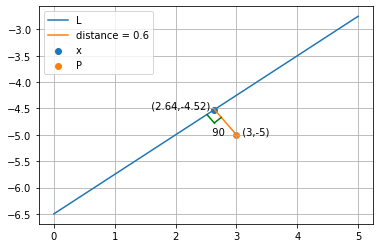
\includegraphics[width=\columnwidth]{./figs/convex_1.2.png}

\item Solve \eqref{eq:opt_line_dist} using cvxpy.
%
\\
\solution  The following code yields
%	
\begin{lstlisting}
codes/line_dist_cvx.py
\end{lstlisting}
%
\begin{align}
\vec{x}_{\min} &= \myvec{2.64\\-4.52},
\\
g\brak{\vec{x}_{\min}} &= 0.6
\end{align}
%

\item Convert  \eqref{eq:opt_line_dist} to an {\em unconstrained} optimization problem.
%
\\
%
\solution $L$ in \eqref{eq:opt_line_nor} can be expressed in terms of the direction vector $\vec{m}$ as
\begin{align}
\label{eq:opt_line_dir}
\vec{x} = \vec{A} + \lambda \vec{m}, 
\end{align}
where $\vec{A}$ is any point on the line and 
%
\begin{align}
\label{eq:opt_line_orth}
\vec{m}^T\vec{n} = 0
\end{align}
%
Substituting \eqref{eq:opt_line_dir} in \eqref{eq:opt_line_dist}, an unconstrained optimization problem 
\begin{align}
\label{eq:opt_line_dist_uncon}
\min_{\lambda}f(\lambda) = \norm{\vec{A} + \lambda \vec{m}-\vec{P}}^2 
\end{align}
%
is obtained.
%
\item Solve \eqref{eq:opt_line_dist_uncon}.
%
\\
\solution 
\begin{align}
f(\lambda) 
& = \brak{ \lambda \vec{m}+\vec{A} -\vec{P}}^T \brak{ \lambda \vec{m}+\vec{A} -\vec{P}}
\\
&= \lambda^2 \norm{\vec{m}}^2 +2\lambda \vec{m}^T\brak{\vec{A} -\vec{P}} 
\nonumber \\
&\quad + \norm{\vec{A} -\vec{P}}^2
\label{eq:opt_line_dist_uncon_dist}
\end{align}
\begin{align}
\because f^{(2)}\lambda = 2\norm{\vec{m}}^2 > 0
\end{align}
%
the minimum value of $f(\lambda)$ is obtained when 
%
\begin{align}
 f^{(1)}(\lambda) &= 2\lambda\norm{\vec{m}}^2 + 2 \vec{m}^T\brak{\vec{A} -\vec{P}} =0
\\
\implies \lambda_{\min} &= -\frac{\vec{m}^T\brak{\vec{A} -\vec{P}}}{\norm{\vec{m}}^2}
\label{eq:opt_line_dist_uncon_lam_min}
\end{align}
%
Choosing $\vec{A}$ such that 
%
\begin{align}
\vec{m}^T\brak{\vec{A} -\vec{P}} &= 0,
\label{eq:opt_line_dist_uncon_trick}
\end{align}
%
substituting in \eqref{eq:opt_line_dist_uncon_lam_min},
%
\begin{align}
\label{eq:opt_line_dist_uncon_lam0}
\lambda_{\min} &= 0 \quad \text{and}
\\
\vec{A} -\vec{P} &= \mu \vec{n}
\label{eq:opt_line_dist_uncon_mu}
\end{align}
for some constant $\mu$. \eqref{eq:opt_line_dist_uncon_mu}
 is a consequence of \eqref{eq:opt_line_orth} and \eqref{eq:opt_line_dist_uncon_trick}. Also, from 
\eqref{eq:opt_line_dist_uncon_mu},
%
\begin{align}
\vec{n}^T\brak{\vec{A} -\vec{P} } &= \mu \norm{\vec{n}}^2
\\
\implies \mu & = \frac{\vec{n}^T\vec{A} -\vec{n}^T\vec{P} }{\norm{\vec{n}}^2} = \frac{c -\vec{n}^T\vec{P} }{\norm{\vec{n}}^2}
\label{eq:opt_line_dist_uncon_mu_sol}
\end{align}
%
from \eqref{eq:opt_line_dist_nor}.
%, where $\mu$ is some constant.
Substituting $\lambda_{\min} = 0$ in \eqref{eq:opt_line_dist_uncon},
%\label
%Thus, the shortest distance from $\vec{P}$ to $L$ is
%
\begin{align}
\min_{\lambda}f(\lambda) =  \norm{\vec{A} -\vec{P}}^2 = \mu^2\norm{\vec{n}}^2
\label{eq:opt_line_dist_uncon_f}
\end{align}
upon substituting from \eqref{eq:opt_line_dist_uncon_mu}. The distance between $\vec{P}$ and ${L}$ is then obtained from \eqref{eq:opt_line_dist_uncon_f} as
% obtained as 
\begin{align}
\norm{\vec{A} -\vec{P}} &= \abs{\mu}\norm{\vec{n}}
\\
&= \frac{\abs{\vec{n}^T\vec{P} -c }}{\norm{\vec{n}}}
\label{eq:opt_line_dist_uncon_f_closed}
\end{align}
after substituting for $\mu$ from  \eqref{eq:opt_line_dist_uncon_mu_sol}. Using the corresponding values from Problem \eqref{prob:opt_line_dist} in \eqref{eq:opt_line_dist_uncon_f_closed},
%
\begin{align}
\min_{\lambda}f(\lambda) =  0.6
\end{align}

%
%
\end{enumerate}
